\documentclass[10pt]{article}

\usepackage[T1]{fontenc}
\usepackage[utf8]{inputenc}
%\usepackage{beton}
%\usepackage{ccfonts}
%\usepackage{concrete}
\usepackage{concmath}
\usepackage{eulervm}
\usepackage{amsmath,amsthm,amssymb}
\usepackage{mathtools}
\usepackage{multicol}
\usepackage{marginnote}
\usepackage{pgfplots}
\usepackage{float}
\usepackage{hyperref}
\usepackage{bbm}
\usepackage{booktabs}
\usepackage{xcolor-solarized}
\usepackage{xcolor}
\usepackage{accents}
\pgfplotsset{compat=1.5}

\usepackage{listings}
\usepackage{xcolor}
\definecolor{codegreen}{rgb}{0,0.6,0}
\definecolor{codegray}{rgb}{0.5,0.5,0.5}
\definecolor{codepurple}{rgb}{0.58,0,0.82}
\definecolor{backcolour}{rgb}{0.95,0.95,0.92}
\lstdefinestyle{mystyle}{
    backgroundcolor=\color{backcolour},   
    commentstyle=\color{codegreen},
    keywordstyle=\color{magenta},
    numberstyle=\tiny\color{codegray},
    stringstyle=\color{codepurple},
    basicstyle=\ttfamily\footnotesize,
    breakatwhitespace=false,         
    breaklines=true,                 
    captionpos=b,                    
    keepspaces=true,                 
    numbers=left,                    
    numbersep=5pt,                  
    showspaces=false,                
    showstringspaces=false,
    showtabs=false,                  
    tabsize=2
}

\lstset{language=Python, style=mystyle}

\usepackage{mathtools}

\usepackage{wasysym}
\usepackage[margin=1.5in]{geometry} 
\usepackage{enumerate}
\index{\usepackage}\usepackage{multicol}

\newcommand{\N}{\mathbf{N}}
\newcommand{\Z}{\mathbb{Z}}

\newcommand{\R}{\mathbf{R}}
\newcommand{\C}{\mathbf{C}}
\newcommand{\Pbb}{\mathbb{P}}
\newcommand{\Fcal}{\mathcal{F}}
\newcommand{\Lcal}{\mathcal{L}}
\newcommand{\Acal}{\mathcal{A}}
\newcommand{\Ecal}{\mathcal{E}}
\newcommand{\Ebb}{\mathbb{E}}
\newcommand{\Qbb}{\mathbb{Q}}


\renewcommand{\mathbf}{\mathbold}

\newenvironment{theorem}[2][Theorem]{\begin{trivlist}
  \item[\hskip \labelsep {\bfseries #1}\hskip \labelsep {\bfseries #2.}]}{\end{trivlist}}
\newenvironment{lemma}[2][Lemma]{\begin{trivlist}
  \item[\hskip \labelsep {\bfseries #1}\hskip \labelsep {\bfseries #2.}]}{\end{trivlist}}
\newenvironment{exercise}[2][Exercise]{\begin{trivlist}
  \item[\hskip \labelsep {\bfseries #1}\hskip \labelsep {\bfseries #2.}]}{\end{trivlist}}
\newenvironment{reflection}[2][Reflection]{\begin{trivlist}
  \item[\hskip \labelsep {\bfseries #1}\hskip \labelsep {\bfseries #2.}]}{\end{trivlist}}
\newenvironment{proposition}[2][Proposition]{\begin{trivlist}
  \item[\hskip \labelsep {\bfseries #1}\hskip \labelsep {\bfseries #2.}]}{\end{trivlist}}
\newenvironment{corollary}[2][Corollary]{\begin{trivlist}
  \item[\hskip \labelsep {\bfseries #1}\hskip \labelsep {\bfseries #2.}]}{\end{trivlist}}

\newenvironment{definition}[2][Definition]{\begin{trivlist}
  \item[\hskip \labelsep {\bfseries #1}\hskip \labelsep {\bfseries #2.}]}{\end{trivlist}}

\definecolor{solar}{rgb}{0.9960, 0.9960, 0.9647}

\begin{document}
  \pagecolor{solar}
	
  \renewcommand{\qedsymbol}{\smiley}
	\title{Investments Class \\ Problem set 9}
	\author{Daniel Grosu, William Martin, Denis Steffen}
		
\maketitle

\begin{exercise}{1}{Mean-variance investing with fixed, linear-proportional, and quadratic trans- action costs}

  To optimize the mean-variance investing for $X_1$, we have two cases because the indicator function is not differentiable. We can define the Lagrangian function as follows:
  $$ \mathcal{L} = \begin{cases}
    X_1\mu - \frac{\gamma}{2}X_1^2\sigma^2 - (b_0 + (X_1-X_0)b_1+\frac{1}{2}\lambda(X_1-X_0)^2), \text{ if } X_1> X_0 \\
    X_1\mu - \frac{\gamma}{2}X_1^2\sigma^2 - (b_0 + (X_0-X_1)b_1+\frac{1}{2}\lambda(X_1-X_0)^2), \text{ if } X_1< X_0
  \end{cases}$$ and so we can differentiate with respect to $X_1$:
  $$ \frac{\partial\mathcal{L}}{\partial X_1} = \begin{cases}
    \mu - \gamma X_1\sigma^2 - (b_1+\lambda(X_1-X_0)), \text{ if } X_1> X_0 \\
    \mu - \gamma X_1\sigma^2 - (- b_1+\lambda(X_1-X_0)), \text{ if } X_1< X_0
  \end{cases}$$

  To find the optimal $X_1$, we equate the two equations to $0$ and find: 
  $$ X_1 = \begin{cases}
    \frac{\mu - b_1 + \lambda X_0}{\gamma\sigma^2+\lambda}, \text{ if } X_1> X_0 \\
    \frac{\mu + b_1 + \lambda X_0}{\gamma\sigma^2+\lambda}, \text{ if } X_1< X_0
  \end{cases}$$

  We know from the lecture course that trading is optimal when $X_0$ does not lie in a no-trade interval that comes from the linear and quadratic transaction costs contraints. Indeed, the linear constraint (alone) gives the no-trade interval $[\frac{\mu- b_1}{\gamma\sigma^2},\frac{\mu+b_1}{\gamma\sigma^2}]$ and the quadratic constraint (alone) gives an optimal value for $X_1 = \frac{\mu+\lambda X_0}{\sigma^2\gamma + \lambda}$. The quadratic constraint does not give any no-trade region as there is a unique solution. So these two constraints give a certain no-trade interval $[\tilde{\underline{X}},\tilde{\overline{X}}]$. 

  In addition, we have a fixed cost constraint and this gives us a second no-trade interval, because we have to make sure that trading is profitable when paying the cost $b_0$ in opposite to not trading. So we have a second interval $[\accentset{\circ}{\underline{X}},\accentset{\circ}{\overline{X}}]$ and then our no-trade region is the domain $ [\tilde{\underline{X}},\tilde{\overline{X}}]\cup [\accentset{\circ}{\underline{X}},\accentset{\circ}{\overline{X}}]$. 

  The fixed cost constraint (only) gives the no-trade interval: $[\frac{\mu}{\sigma^2\gamma} -\sqrt{\frac{2b_0}{\gamma\sigma^2}},\frac{\mu}{\sigma^2\gamma} +\sqrt{\frac{2b_0}{\gamma\sigma^2}}]$. And we can see that the number $\frac{\mu}{\sigma^2\gamma}$ is in the two intervals, so they are not disjoint. 
  
  Thus the no-trade region is an interval $[\underline{X},\overline{X}]$ depending on the parameters, $\mu, b_0, b_1,\gamma, \lambda$ and $\sigma^2$. 

  Now we need to compute the trading speed and the aim portfolio such that: $X_1 = \tau aim + (1-\tau)X_0$

\end{exercise}

\newpage

\begin{exercise}{2}
\end{exercise}

a) We solve for the optimal portfolio when there is one single risky asset and the risk-less asset. Thus, maximizing the mean-variance objective function gives us the optimal portfolio (one dimensional) if we decide to long the risky asset $X_1$:

\begin{align*}
	max \quad C(X_1) = R_f + X_1(\mu - R_f) - \frac{\gamma}{2} \Sigma X_1^2 - (X_1 - X_0)b
\end{align*}

Solving for the optimal portfolio $X_1^*$ 

\begin{align*}
	& \mu - R_f - \gamma \Sigma X_1^* - b = 0 \\
	& X_1^* = \frac{1}{\gamma} \Sigma^{-1} (\mu - R_f  - b)
\end{align*}

If it is optimal from the initial dollar position $X_0$ to buy more of $X_1$, then this can be done as long as as $X_0 < X_1^*$. We thus have $X_1^* = X_L$ where we should trade. In other words

\begin{align*}
	X_0 < X_L = \frac{1}{\gamma} \Sigma^{-1} (\mu - R_f  - b)
\end{align*}

Shorting $X_1$ is equivalent to maximizing the following mean-variance objective function:

\begin{align*}
	max \quad C(X_1) = R_f + X_1(\mu - R_f) - \frac{\gamma}{2} \Sigma X_1^2 - (-X_1 + X_0)b
\end{align*}

Computing the first order condition with respect to $X_1$ gives us:

\begin{align*}
	X_1^* =\frac{1}{\gamma} \Sigma^{-1} (\mu - R_f + b)
\end{align*}

Similarly, we can sell the risky asset $X_1$ from initial dollar position $X_0$ as long as $X_0 > X_1^*$, which gives us $X_h$:

\begin{align*}
	X_0 > X_h = \frac{1}{\gamma} \Sigma^{-1} (\mu - R_f + b)
\end{align*}

The no-trade region is thus the inverse of the optimal trading region, that is $X_0 \in [X_l, X_h]$, where we should not trade.

\bigbreak

b) With two assets to trade, we can draw all trade possibilities in a table:

\begin{center}
\begin{tabular}{|l|c|c|c|}
\hline
           & \multicolumn{1}{l|}{buy 1} & \multicolumn{1}{l|}{no trade 1} & \multicolumn{1}{l|}{sell 1} \\ \hline
sell 2      & bs  & ns & ss \\ \hline
no trade 2 & bn  & nn & sn \\ \hline
buy 2     & bb & nb & sb  \\ \hline
\end{tabular}
\end{center}

The no-trade region is thus, similarly to a), the inverse region of the do-trade region defined by the sets $\{bb, bn, bs, nb, ns, sb, sn, ss\}$. We thus need to define these 8 regions first in order to define the no-trade region.

\smallbreak

We need to control the sign of each component of $(X_1 - X_0)^T$. To this end we introduce the diagonal matrix \textbf{A}:

\begin{align*}
	A = \begin{pmatrix}
a_{1} & 0\\
0 & a_{2}
\end{pmatrix}
\end{align*}

Where components $a_{11}$ and $a_{22}$ can either take values -1, 1 or 0 to emulate either a sell, buy or no-trade position of each risky asset. We can therefore rewrite the objective function as follows

\begin{align*}
	max \quad C(X_1) = R_f  + X_1^T(\mu - R_f)  - \frac{\gamma}{2} X_1^T \Sigma X_1  - (X_1  - X_0)^TAb
\end{align*}

Taking the first case of the table, that is buy risky asset 1 and 2 ($bb$) and maximizing the modified mean-variance objective function, taking the first order condition: 

\begin{align*}
	& \mu - R_f - \gamma \Sigma X_1 - Ab = 0\\
	& X_{bb} = X_1^*(A) = \frac{1}{\gamma}\Sigma^{-1} (\mu - R_f - Ab)
\end{align*}

Where 

\begin{align*}
	A = \begin{pmatrix}
	1 & 0\\	
	0 & 1
\end{pmatrix}
\end{align*}

Let us denote by $X_0^1$ and $X_0^2$ the initial dollar position of the first and second risky assets respectively and similarly $X_1^1$ and $X_1^2$ their final dollar position. The optimal trading region for the $bb$ case is thus when $bb = \{ X_0 \in \mathbb{R}^2 \vert X_0^1 < X_{bb}^1 \cap  X_0^2 < X_{bb}^2\}$.

\bigbreak

The other 3 corners of the table can be expressed by following the same procedure. For the $sb$ case. We have 

\begin{align*}
	X_{sb} &= X_1^*(A) \\
	A &=  \begin{pmatrix}
	-1 & 0\\	
	0 & 1
\end{pmatrix}
\end{align*}

Therefore $sb = \{X_0 \in \mathbb{R}^2 \vert X_0^1 > X_{sb}^1 \cap  X_0^2 < X_{sb}^2\}$. For the $bs$ case we have 

\begin{align*}
		X_{bs} &= X_1^*(A) \\
	A &=  \begin{pmatrix}
	1 & 0\\	
	0 & -1
\end{pmatrix}
\end{align*}

Therefore $bs = \{X_0 \in \mathbb{R}^2 \vert X_0^1 < X_{bs}^1 \cap  X_0^2 > X_{bs}^2\}$. Finally for the $ss$ case we have 

\begin{align*}
		X_{ss} &= X_1^*(A) \\
	A &=  \begin{pmatrix}
	-1 & 0\\	
	0 & -1
\end{pmatrix}
\end{align*}

Therefore $ss = \{ X_0 \in \mathbb{R}^2 \vert X_0^1 > X_{ss}^1 \cap  X_0^2 > X_{ss}^2\}$.

\bigbreak

We now need to defined the trading regions where only one risky asset is traded. For the $bn$ case, we leave the second risky asset untouched, that is $X_1^2 = X_0^2$: its final and initial dollar positions are identical. The modified mean-variance objective function to maximize becomes the following ($a_1 = 1$ and $a_2 = 0$ in the matrix $A$)

\begin{align*}
	max \quad C(X_1^1) &= R_f + X_1^T(\mu - R_f) - \frac{\gamma}{2}X_1^T\Sigma X_1 - (X_1 - X_0)^T \begin{pmatrix}
	1 & 0\\	
	0 & 0
\end{pmatrix} b \\
&= R_f + X_1^1(\mu_1 - R_f) + X_0^2(\mu_2 - R_f) - \frac{\gamma}{2}  \begin{pmatrix}
	X_1^1 & X_0^2
\end{pmatrix} \begin{pmatrix}
	\sigma_1^2 & \rho \sigma_1 \sigma_2\\	
	\rho \sigma_1 \sigma_2 & \sigma_2^2
\end{pmatrix} \begin{pmatrix}
	X_1^1 \\	
	X_0^2 
\end{pmatrix} \\
& - \begin{pmatrix}
	X_1^1 - X_0^1 & X_0^2 - X_0^2
\end{pmatrix} \begin{pmatrix}
	b_1 \\	
	0 
\end{pmatrix}\\
&= R_f + X_1^1(\mu_1 - Rf - b_1) + X_0^2(\mu_2 - R_f) - \frac{\gamma}{2}\left( X_1^1 X_1^1 \sigma_1^2 + X_0^2 X_0^2 \sigma_2^2 + 2 X_1^1X_0^2\rho \sigma_1 \sigma_2 \right)\\
	& + X_0^1b_1
\end{align*}

Taking the first order condition with respect to $X_1^1$ gives us

\begin{align*}
	& \mu_1 - R_f - b_1 - \gamma X_1^1\sigma_1^2 - \gamma X_0^2 \rho \sigma_1 \sigma_2 = 0	\\
	& X_{bn}^1(X_0^2) =  X_1^{1*}(X_0^2)  = \frac{\mu_1 - R_f - b_1}{\gamma \sigma_1^2} - \frac{X_0^2 \rho  \sigma_2}{\sigma_1} 
\end{align*}

Moreover, since we are not trading risky asset 2, this must mean that for the  $bn$ case it must be in the no-trade region knowing that risky asset 1 is in a long position: $X_{bb}^2 \leq X_0^2 \leq X_{bs}^2$ (result similar to the first part $a$). The  set $bn $ is thus the intersection between not trading risky asset 2 (conditional on longing risky asset 1) and buy risky asset 1 (conditional on not trading risky asset 2) until reaching $X_{bn}^1(X_0^2)$. Therefore, $bn = \{ X_0 \in \mathbb{R}^2 \vert X_{bb}^2 \leq X_0^2 \leq X_{bs}^2 \cap X_0^1 < X_{bn}^1(X_0^2) \}$.

\bigbreak

We can derive similar results for the other 3 quadrants of the table, where one risky asset is traded and the other risky asset is not traded. For $sn$, we optimally sell risky asset 1 and don't trade risky asset 2

\begin{align*}
	X_{sn}^1(X_0^2) =  X_1^{1*}(X_0^2)  = \frac{\mu_1 - R_f + b_1}{\gamma \sigma_1^2} - \frac{X_0^2 \rho  \sigma_2}{\sigma_1}
\end{align*}

Following the same argument than for $bn$, we obtain the set $sn = \{ X_0 \in \mathbb{R}^2 \vert X_{sb}^2 \leq X_0^2 \leq X_{ss}^2 \cap X_0^1 > X_{sn}^1(X_0^2) \}$. For $nb$, we optimally buy risky asset 2 while not trading risky asset 1

\begin{align*}
	X_{nb}^2(X_0^1) =  X_1^{2*}(X_0^1)  = \frac{\mu_2 - R_f - b_2}{\gamma \sigma_2^2} - \frac{X_0^1 \rho  \sigma_1}{\sigma_2}
\end{align*}

The set is thus $nb = \{X_0 \in \mathbb{R}^2 \vert X_{bb}^1 \leq X_0^1 \leq X_{sb}^1 \cap X_0^2 < X_{nb}^2(X_0^1) \}$.

For $ns$, we optimally sell risky asset 2 while not trading risky asset 1

\begin{align*}
	X_{ns}^2(X_0^1) =  X_1^{2*}(X_0^1)  = \frac{\mu_2 - R_f + b_2}{\gamma \sigma_2^2} - \frac{X_0^1 \rho  \sigma_1}{\sigma_2}
\end{align*}

The set is thus $ns = \{ X_0 \in \mathbb{R}^2 \vert X_{bs}^1 \leq X_0^1 \leq X_{ss}^1 \cap X_0^2 > X_{ns}^2(X_0^1) \}$.

\bigbreak

Finally the no-trade region is the inverse of all trading regions. That is 

\begin{align*}
	nn = \{ X_0 \in \mathbb{R}^2 \textbackslash (bb \cup sb \cup bs \cup ss \cup bn \cup sn \cup nb \cup ns) \}
\end{align*}

Plotting the optimal trading regions gives us figure \ref{ex2_1}, the no-trading region being a parallelogram: 

\begin{figure}[h]
    \centering
    \makebox[\linewidth][c]{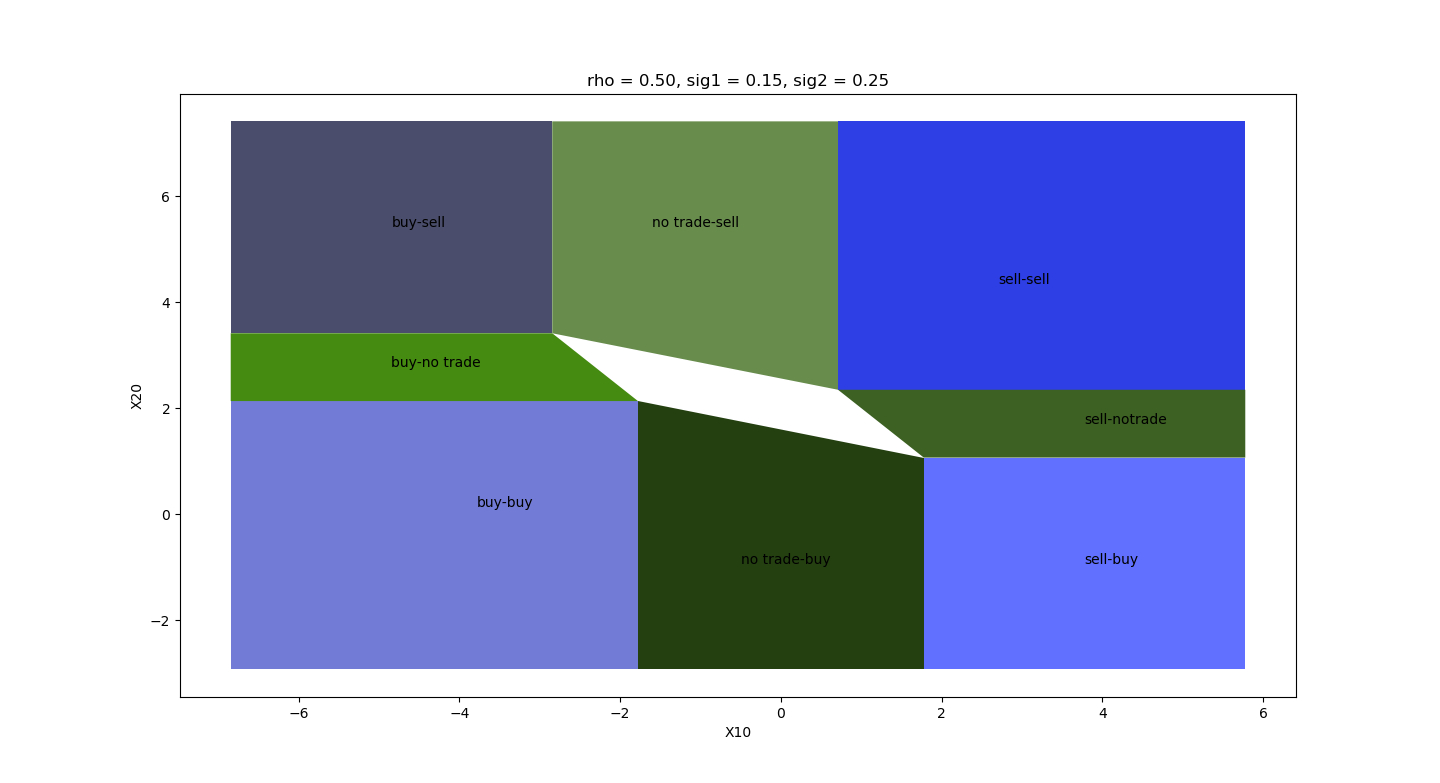
\includegraphics[scale=0.5]{ex2_1.png}}
    \caption{Optimal trading regions}
    \label{ex2_1}    
\end{figure}

\bigbreak

c) As we increase the correlation coefficient $\rho$ between the two assets, we obtain figure \ref{ex2_2}, the no-trading region starts by being a rectangle and flattens into a parallelogram until it completely vanishes.

\begin{figure}[h]
    \centering
    \makebox[\linewidth][c]{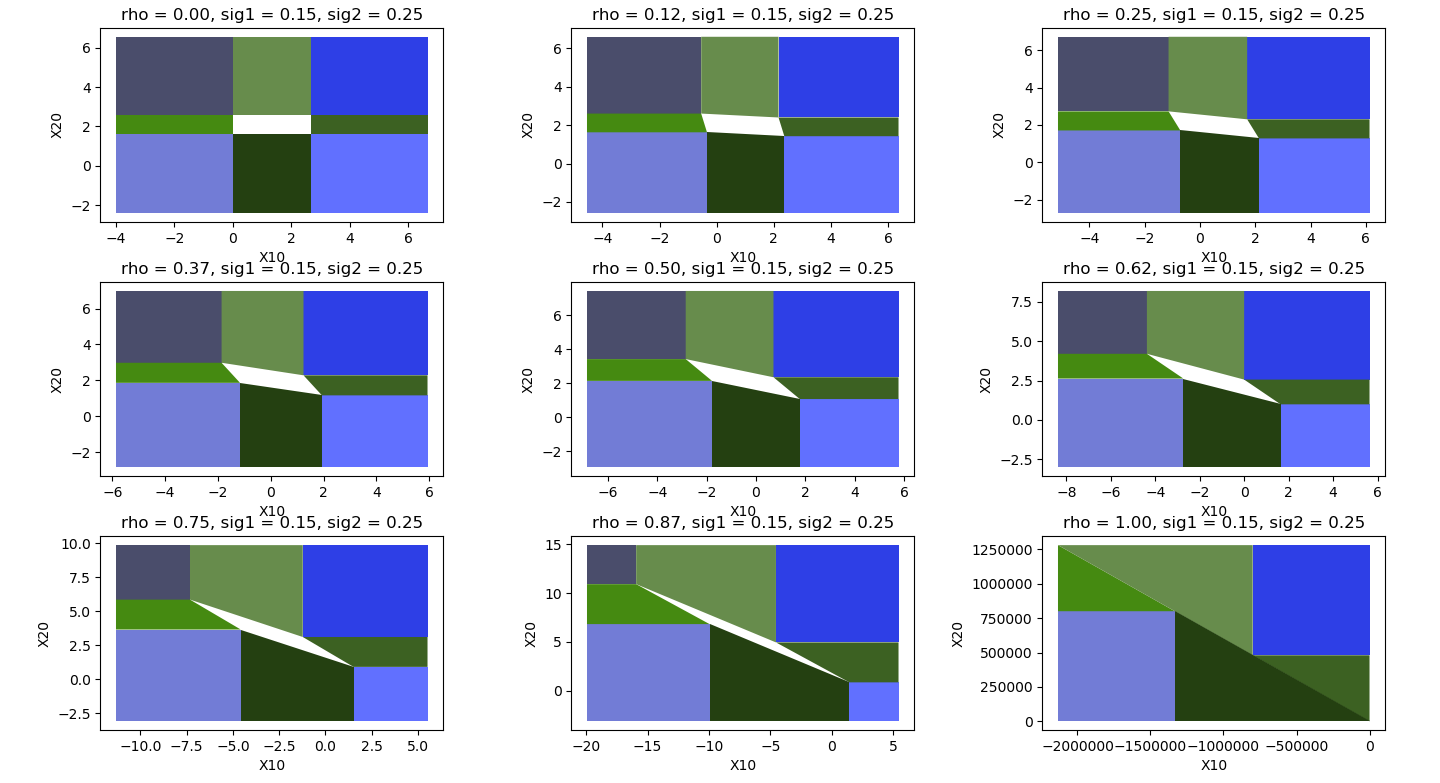
\includegraphics[scale=0.5]{ex2_2.png}}
    \caption{Optimal trading regions as $\rho$ increases}
    \label{ex2_2}    
\end{figure}

As we increase the voltatility of asset 2, we obtain figure \ref{ex2_3}. The $bn$,$sn$, and no trade regions become slimmer. On the other hand, the $bs$, $bb$, $ss$, and $sb$ regions become larger.

\begin{figure}[h]
    \centering
    \makebox[\linewidth][c]{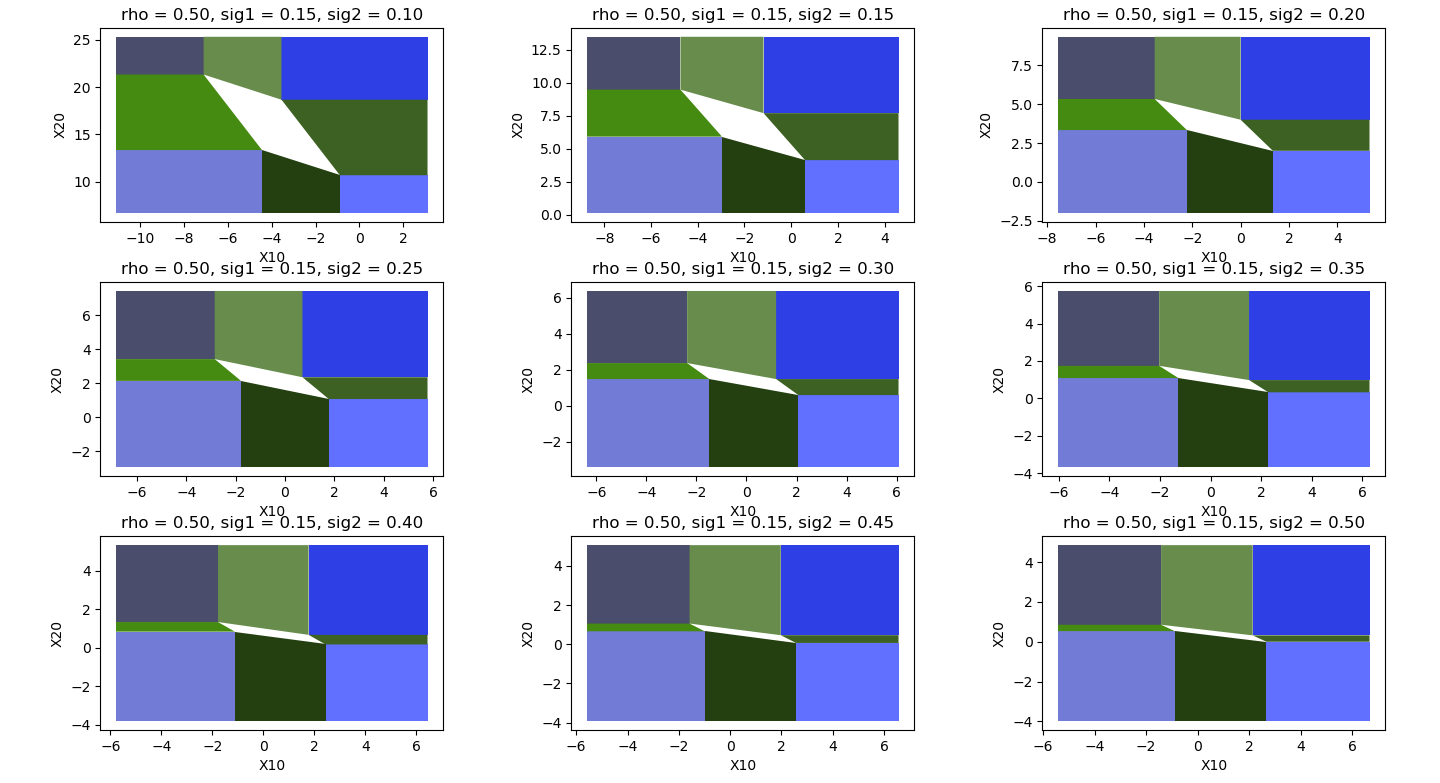
\includegraphics[scale=0.5]{ex2_3.png}}
    \caption{Optimal trading regions as $\sigma_2$ increase}
    \label{ex2_3}   
\end{figure}

\newpage

\begin{exercise}{3}{Optimal Dynamic trading of a single asset with linear-proportional price impact (quadratic transaction costs)}

  \begin{itemize}
    \item
    The value function with trading costs at time $T$ is
    \begin{align*}
      V(T, n_{T - 1}) &= \Ebb\left[ \sum_{t = T}^T \gamma^{t - T}\left\{ n_t\mu -
      \frac \lambda 2 \left( n_t - n_{t - 1} \right)^2 + \frac \gamma 2
      n_t^2\sigma^2 \right\} \right]  \\
      &= n_T\mu -
      \frac \lambda 2 \left( n_T - n_{T - 1} \right)^2 + \frac \gamma 2
      n_T^2\sigma^2.  \\
    \end{align*}
  Solving the First-Order condition with respect to $n_{T}$ yields the solution
  to the last period maximization problem:
  \begin{align*}
    \frac{\partial V(T, n_{T - 1})}{\partial n_T} = \mu - \lambda (n_T -
    n_{T-1}) + \gamma n_T \sigma^2 = 0
  \end{align*}
  which solves to
  \begin{align*}
    n_T = \frac{\mu + \lambda n_{T-1}}{\lambda + \gamma \sigma^2} = n^*(T, n_{T
    - 1})
  \end{align*}
  The solution $n^*(T, n_{T-1})$ is indeed a maximum since $\frac{\partial^2 V(T,
    n_{T-1})}{\partial n_T^2} = -\lambda - \gamma < 0$. The value function at
  the maximizer evaluates to:

  \begin{align*}
    V^*(T, n_{T-1}) &= n^*(T, n_{T-1})\mu - \frac \lambda 2 \left(n^*(T, n_{T - 1}) -
    n_{T-1}\right)^2 - \frac \gamma 2 n^*(T, n_{T-1})^2 \sigma^2 \\
    &= \frac{\mu + \lambda n_{T-1}}{\lambda + \gamma \sigma^2}\mu - \frac \gamma
      2 \left( \frac{\mu + \lambda n_{T-1}}{\lambda + \gamma \sigma^2} - n_{T-1}\right)^2 - \frac
      \gamma 2 \left(\frac{\mu + \lambda n_{T-1}}{\lambda + \gamma \sigma^2} \right) ^2
      \sigma^2 \\
    &= \frac{\mu + \lambda n_{T-1}}{\lambda + \gamma \sigma^2}\mu - \frac \gamma
      2 \left( \frac{\mu - \gamma\sigma^2n_{T-1}}{\lambda + \gamma \sigma^2}\right)^2 - \frac
      \gamma 2 \left(\frac{\mu + \lambda n_{T-1}}{\lambda + \gamma \sigma^2} \right) ^2
      \sigma^2 \\
    &= \frac{\mu^2 + \lambda n_{T-1} \mu}{\lambda + \gamma \sigma^2} - \frac \gamma
      2 \frac{\mu^2 - 2\mu\gamma\sigma^2n_{T-1} + \gamma^2\sigma^4n_{T-1}^2}{(\lambda + \gamma \sigma^2)^2} - \frac
      \gamma 2 \frac{\mu^2 + 2\mu\lambda n_{T-1} + \lambda^2 n_{T-1}^2}{(\lambda + \gamma \sigma^2)^2}
      \sigma^2 \\
    &= \frac{\mu^2(\lambda \gamma\sigma^2) - \frac\lambda 2 \mu^2 - \frac \gamma
      2 \mu^2\sigma^2}{(\lambda  + \gamma\sigma^2)^2} + \\
      & \;\;\;\; + \frac{\lambda\mu n_{t-1} (\lambda + \gamma \sigma^2) +
        \lambda\mu n_{T-1}\gamma \sigma^2 - \gamma \lambda
        n_{T-1}\sigma^2}{(\lambda + \gamma \sigma ^2)^2} +  \\
        & \;\;\;\; + \frac 1 2 \frac{n_{T-1}^2 (\gamma \sigma ^2 ( - \lambda \gamma
          \sigma^2 - \lambda ^ 2))}{(\lambda + \gamma \sigma^2)^2}\\
    &= \frac{\frac 1 2 \mu^2 (\lambda + \gamma \sigma^2)}{(\lambda  + \gamma\sigma^2)^2} 
       + \frac{\lambda\mu n_{t-1} (\lambda + \gamma \sigma^2)} {(\lambda + \gamma \sigma ^2)^2}  
         - \frac 1 2 \frac{n_{T-1}^2 (\lambda \gamma \sigma ^2 ( \gamma
          \sigma^2 + \lambda))}{(\lambda + \gamma \sigma^2)^2}\\
    &= \frac{\frac 1 2 \mu^2}{(\lambda  + \gamma\sigma^2)} 
       + \frac{\lambda\mu n_{t-1}} {(\lambda + \gamma \sigma ^2)} 
         - \frac 1 2 \frac{n_{T-1}^2 \lambda \gamma \sigma ^2}{(\lambda + \gamma \sigma^2)}\\
         &= - \frac 1 2 \frac{ \lambda \gamma \sigma ^2}{\lambda + \gamma
           \sigma^2} n_{T-1}^2 
        + \frac{\lambda\mu }{\lambda + \gamma \sigma ^2}n_{t-1}
        + \frac 1 2 \frac{\mu^2}{\lambda  + \gamma\sigma^2}.  \\
  \end{align*}
  The constants are then read to be
  \begin{align*}
    Q_T = \frac{\lambda\gamma\sigma^2}{\lambda + \gamma\sigma^2}, \\
    q_T = \frac{\lambda \mu}{\lambda + \gamma\sigma^2}, \\
    c_T = \frac 1 2 \frac{\mu^2}{\lambda + \gamma \sigma^2}.
  \end{align*}

  \item
    The Bellman equation
    \begin{align*}
      V(t, n_{t - 1}) = max_{n_t}\left\{ n_t\mu - \lambda 2 (n_t - n_{t-1})^2
      \frac \gamma 2 n_t^2 \sigma^2 + \rho \Ebb_t\left[ V(t+1, n_t) \right] \right\}
    \end{align*}
    under the assumption that the value function $V(t +1, n_t)$ is a quadratic
    form:
    \begin{align*}
      V(t+1, n_t) = - \frac 1 2 Q_{t+1}n_{t} + q_{t+1}n_t + c_{t + 1},
    \end{align*}
    reduces to the following maximization problem:
    \begin{align*}
      V(t, n_{t-1}) = \max_{n_t}\left\{ n_t \mu - \frac \lambda 2 (n_t -
      n_{t-1})^2 - \frac \gamma 2 n_t^2 \sigma^2 - \gamma \frac 1 2 n_t^2
      Q_{t+1} + \rho n_t q_{t+1} + \rho c_{t+1} \right\}.
    \end{align*}
    Once again, the First-order condition is:
    \begin{align*}
      \frac{\partial V(t,n_{t-1})}{\partial n_t} = \mu - \lambda(n_t - n_{t-1})
      - \gamma n_t \sigma^2 - \rho n_t Q_{t+1} + \rho q_{t+1} = 0,
    \end{align*}
    which solves to the optimum
    \begin{align*}
      n_t^* = \frac{\mu + \lambda n_{t-1} + \rho q_{t+1}}{\lambda + \gamma\sigma^2+ \rho Q_{t+1}}.
    \end{align*}

    Plugging it back in the value function, we have that
    \begin{align*}
      V(t, n_{t - 1}) &= \frac{\mu + \lambda n_{t-1} + \rho q_{t+1}}{\lambda + \gamma\sigma^2+ \rho Q_{t+1}}(\mu + \rho q_{t+1}) \\
      & \;\;\;\; - \frac \lambda 2
      \frac{(\mu + \rho q_{t+1} - n_{t-1}(\gamma\sigma^2 + \rho Q_{t+1}))^2}{(\lambda + \gamma\sigma^2+ \rho Q_{t+1})^2}  \\
      & \;\;\;\; + \left( \frac{\mu + \lambda n_{t-1} + \rho q_{t+1}}{\lambda + \gamma\sigma^2+ \rho Q_{t+1}}
 \right)^2\left( - \frac 1 2 \gamma \sigma^2 - \frac 1 2 \rho Q_{t + 1} \right) \\
      &= \frac{(\mu  + \rho q_{t+1})+ \lambda n_{t-1}}{\lambda + (\gamma\sigma^2+ \rho Q_{t+1})}(\mu + \rho q_{t+1}) \\
      & \;\;\;\; - \frac \lambda 2
      \frac{((\mu + \rho q_{t+1}) - n_{t-1}(\gamma\sigma^2 + \rho Q_{t+1}))^2}{(\lambda + (\gamma\sigma^2+ \rho Q_{t+1}))^2}  \\
      & \;\;\;\; - \frac 1 2\left( \frac{(\mu + \rho q_{t+1}) + \lambda n_{t-1}}{\lambda + (\gamma\sigma^2+ \rho Q_{t+1})}
 \right)^2\left(\gamma \sigma^2 + \rho Q_{t + 1} \right).
    \end{align*}
    Notice that the algebra of this expression is congruent to the one of the
    last period ($V(T, n_{T-1})$) up to the following substitution:
    \begin{align*}
      \mu &\mapsto \mu + \rho q_{t+1} \\
      \gamma\sigma^2 &\mapsto \gamma\sigma^2 + \rho Q_{t+1}
    \end{align*}
    As such, we can use the previous results and perform the above substitutions
    to get the following results:
    \begin{align*}
      Q_t &= \frac{(\gamma \sigma^2 + \rho Q_{t+1})\lambda}{\lambda + \gamma\sigma^2 + \rho Q_{t+1}}, \\
      q_t &= \frac{\lambda(\mu + \rho q_{t+1})}{\lambda + \gamma \sigma^2 + \rho Q_{t+1}}, \\
      c_t &= \frac 1 2 \frac{(\mu + \rho q_{t+1})^2}{\lambda + \gamma \sigma^2 + \rho Q_{t+1}} + \rho c_{t+1}.
    \end{align*}

    \item
      The portfolio $aim_{t}$ maximizes the value function at any time $t$ in
      absence of trading costs. That is, the FOC condition respected by obeyed
      by $aim_t$ is ($\lambda = 0$):

      \begin{align*}
      \frac{\partial V(t,n_{t-1})}{\partial n_t} = \mu - \gamma n_t \sigma^2 - \rho n_t Q_{t+1} + \rho q_{t+1} = 0
      \end{align*}
      and
      \begin{align*}
        aim_t = \frac{\mu + \rho q_{t+1}}{\gamma\sigma^2 + \rho Q_{t+1}}.
      \end{align*}

      The optimum strategy $n_{t+1}$ can be written as:

      \begin{align*}
        n_{t+1} &= \frac{\mu + q_{t+2}}{\lambda + \gamma \sigma^2 + Q_{t+2}} + \frac{\lambda n_t}{\lambda + \gamma\sigma^2 + Q_{t+2}} \\
        &= \left(1 - \frac{\gamma\sigma^2 + Q_{t+2}}{\lambda + \gamma\sigma^2 + Q_{t+2}} n_t \right) + \frac{\mu + q_{t+2}}{\lambda + \gamma \sigma^2 + Q_{t+2}} \\
        &= \left(1 - \frac{\gamma\sigma^2 + Q_{t+2}}{\lambda + \gamma\sigma^2 + Q_{t+2}} n_t \right) + \frac{\gamma\sigma^2 + \rho Q_{t+2}}{\lambda + \gamma \sigma^2 + Q_{t+2}}\frac{\mu + q_{t+2}}{\gamma\sigma^2 + \rho Q_{t+2}}  \\
      \end{align*}
      which assumes the form $n_{t+1} = (1 - \tau_t) n_t + \tau_t aim_t$ for
      \begin{align*}
        \tau_t = \frac{\gamma\sigma^2 + \rho Q_{t+2}}{\lambda + \gamma \sigma^2 + Q_{t+2}} \;\;\;  \text{ and } \;\;\;
        aim_t = \frac{\mu + \rho q_{t+1}}{\gamma\sigma^2 + \rho Q_{t+1}}.
      \end{align*}

      \item
        The situation we are presented in this case involves a portfolio
        consisting solely of shares of a single stock which are essentially
        worthless from the point of view of investment opportunities ($\mu =
        0$), not delivering their holder any capital or dividend gains. Surely
        in case when the mean-variance investor can find zero risk investments
        with positive yield (such as a positive risk-free rate), he will choose
        to liquidate this portfolio. Therefore, at time T the investor will want
        to hold zero shares of the asset.
        The fact that at time T the investor would rather hold zero shares is
        also a property intrinsic in the model: since our model is
        finite-horizon, there is no utility to be gained beyond the $T$'th
        period hence the investor may as well sell his shares at any
        non-negative price. But wanting to liquidate the portfolio will not
        always mean that he will also be able to: the trading fees may be high
        enough that the cost of the transaction exceeds the market price of the
        share, rendering the deal unjustified.

        We choose the parameters for the model as follows:
        \begin{align*}
          \mu &= 0 \\
          \gamma &= 0 \\
          \lambda_t &= \begin{cases} 2 bps & \text{if } 2.5 <= t <= 4.5 \\ 1 bps & \text{otherwise} \end{cases} \\
          \sigma_{annually} = 30 \%
        \end{align*}
        where $t$ is the elapsed time in hours since the opening of
        the exchange on a given trading day. The annualized volatility will need
        to be converted into 30 minutes and 10 minutes volatility for our
        application. We do it directly in the application assuming that most
        years contain 252 trading days and each trading day affords 6.5 trading
        hours (from 09:30AM to 04:00PM).

        \begin{align*}
          \sigma_{daily} &= \frac{\sigma_{annually}}{\sqrt{252}} \\
          \sigma_{30min} &= \frac{\sigma_{daily} }{\sqrt{13}} \\
          \sigma_{10min} &= \frac{\sigma_{daily} }{\sqrt{39}}
        \end{align*}

        Between $09:30AM$ and $04:00PM$ there are 13 30-minute intervals and $3
        \times 13 = 39$ 10-minute intervals. The 30-minute model will therefore
        contain 14 periods and the 10-minute model 40 periods.
        \begin{figure}[H]
          \centering
          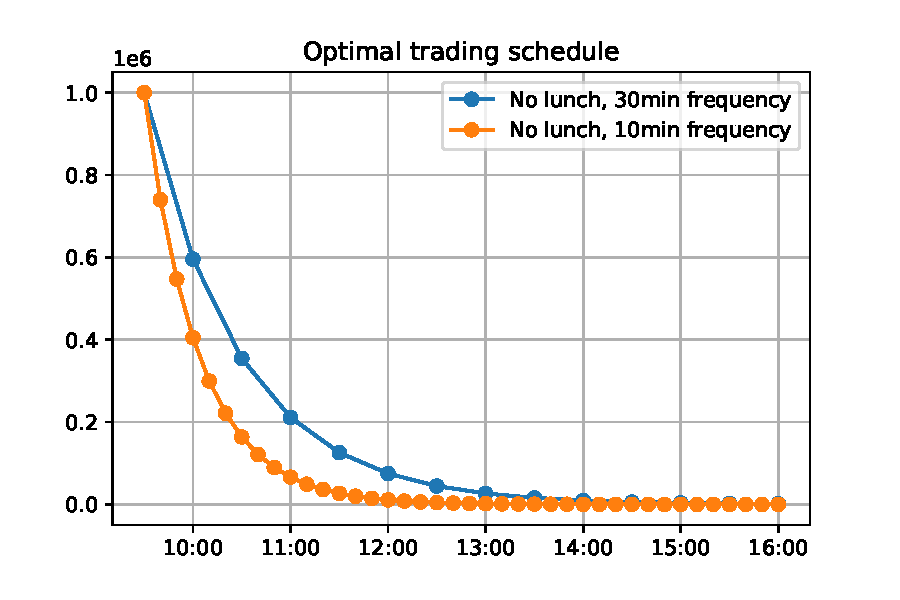
\includegraphics[scale=0.6]{fig1.pdf}
          \caption{The optimal holding portfolio as a function of time in the
            case of a trading frequency of 30 minutes and 10 minutes}
          \label{fig:fig1}
        \end{figure}

        The \autoref{fig:fig1} renders the optimal trading schedule of a trader
        who trades every 30 or 10 minutes. The more frequent trader is able to
        liquidate the portfolio at a higher speed than his slower counterpart.
        
        
        \begin{figure}[H]
          \centering
          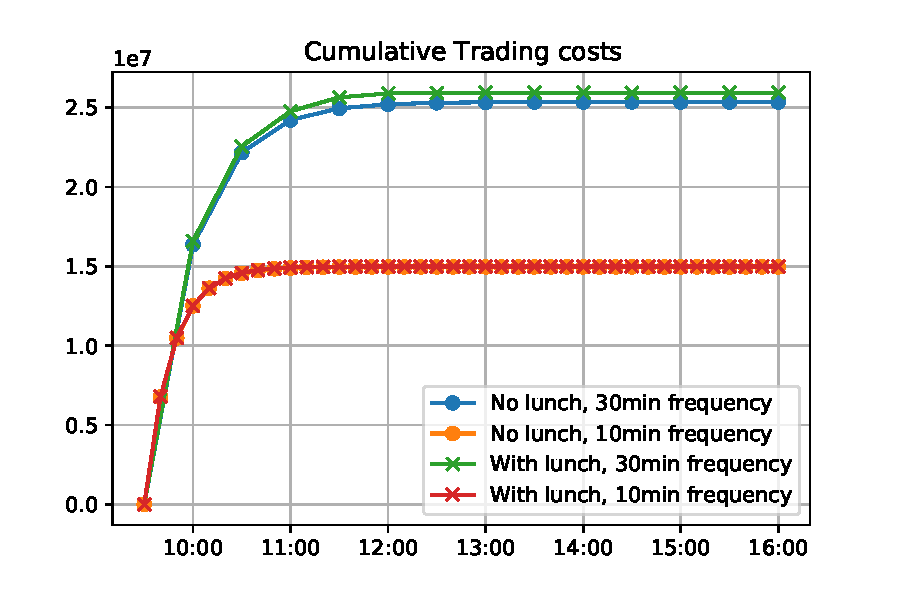
\includegraphics[scale=0.6]{fig2.pdf}
          \caption{Cumulative trading costs as a function of time in the
            case of a trading frequency of 30 minutes and 10 minutes and whether the
          ``trader's lunch'' is taken into account or not.}
          \label{fig:fig2}
        \end{figure}
        In \autoref{fig:fig2}, the cumulative trading costs substantiates our
        expectations that most costs will be incured in the first large trades.


        
        \begin{figure}[H]
          \centering
          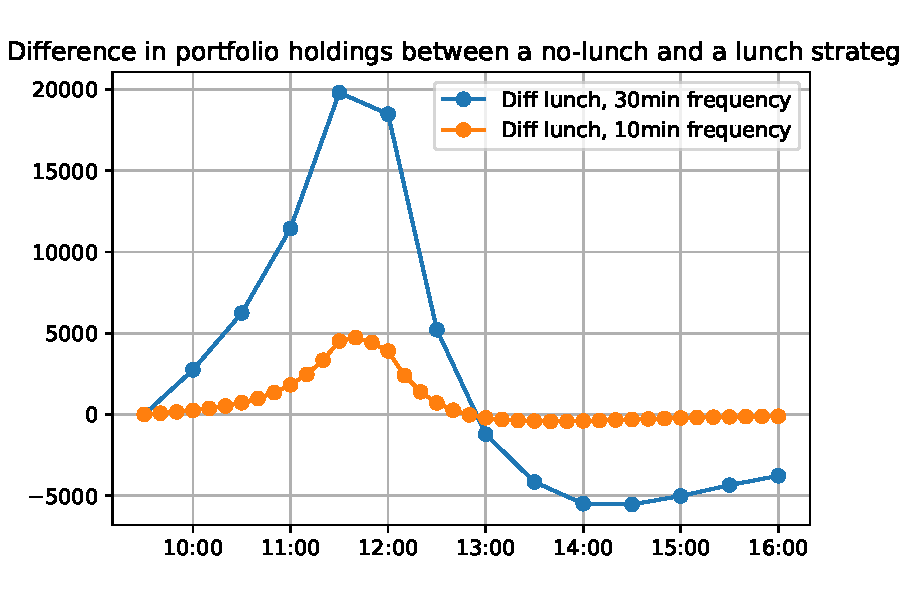
\includegraphics[scale=0.6]{fig3.pdf}
          \caption{The difference in the portfolio holdings between the
            portfolio of a trader who doesn't take into account and one that
            takes into account the ``trader's lunch'' (for 30-minute and
            10-minute frequency).}
          \label{fig:fig3}
        \end{figure}

        In \autoref{fig:fig3} it is observed that the trader that doesn't take
        into account the heightened illiquidity between 12:00PM and 02:00PM will
        have a higher holding of shares than the one that does take it into
        account. This of course implies that the trader facing heightened illiquidity
        at lunch will optimally have to sell more shares before the lunch. For
        the more frequent trader, higher trading costs do not seem to impact
        markedly his optimal trading portfolio, presumably owing to his ability
        to trade often and in small portions, paying less cumulative costs overall.


        \item
          The model predicts that the optimal trading schedule does not depend
          on the realized price shocks, that is, if the stock price goes up over
          the trading day or if it goes down does not affect the overall optimal
          trading rule. This is of course preposterous. As an investor, you
          would like to get out of a trade with as much cash in your hand as possible so you
          would avoid trading if the price is too low, perhaps spreading out the
          liquidation of the portfolio over a couple of days. This is especially
          crucial if our portfolio consists of a large portion of a stock's
          total number of outstanding shares (such as Buffett's airlines
          portfolio) in which case a precipitate sell-off can turn the market
          against the trader.

          The model
          assumes that we do not derive any utility from the price at which we sell off the
          shares and therefore only tries to minimize the disutility of trading
          costs. In order to change the optimal trading rule so that it accounts
          for the price shocks, we can introduce a positive utility term in the
          value function
          representing the cash we get back for selling a part of shares:
          \begin{align*}
            c \times P_t \times (n_{t - 1} - n_t)
          \end{align*}
  \end{itemize}
  
\end{exercise}
   
\end{document}



\appendix


